\section{细胞吸入微管道的模拟}

\subsection{细胞的DPD模型}
\frame{\frametitle{FENE模型}
耗散粒子动力学模拟DNA等生物高分子流
动时, 一般采用珠簧链模型, 两个珠子之间
的弹簧力表达式为
\begin{columns}
  \begin{column}[b]{0.5\textwidth}
\begin{center}
 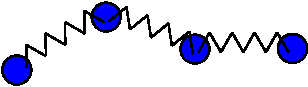
\includegraphics[width=0.6\textwidth]{FENE.pdf}
\end{center}
  \end{column}

  \begin{column}[b]{0.5\textwidth}
\[
\mathbf{F}_{ij}^S = \frac{H\mathbf{r}_ij}{1-(r_{ij}/r_{\max})^2}
\]
  \end{column}

\end{columns}
}

\frame{\frametitle{细胞的构造}
细胞膜的构造是通过FENE模型中的弹簧力将DPD粒子串联成球

  \begin{columns}
  \begin{column}[b]{0.33\textwidth}
\begin{center}
 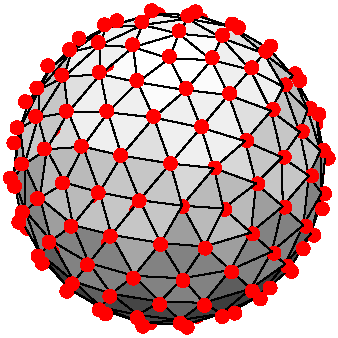
\includegraphics[width=0.8\textwidth]{p162.pdf}

$N = 162$
\end{center}
  \end{column}
  \begin{column}[b]{0.33\textwidth}
\begin{center}
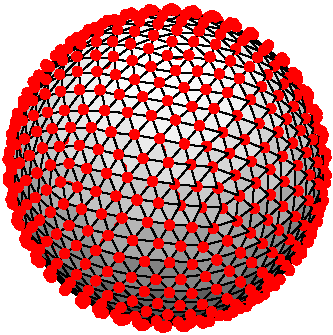
\includegraphics[width=0.8\textwidth]{p642.pdf}

$N=642$
\end{center}
  \end{column}
  \begin{column}[b]{0.33\textwidth}
\begin{center}
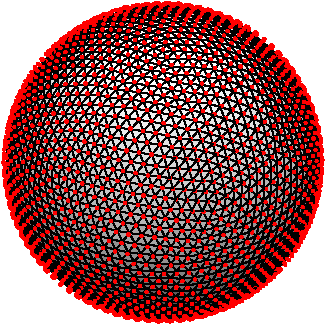
\includegraphics[width=0.8\textwidth]{p2562.pdf}

$N=2562$
\end{center}
  \end{column}
\end{columns}
}
\frame{\frametitle{模拟示意图}
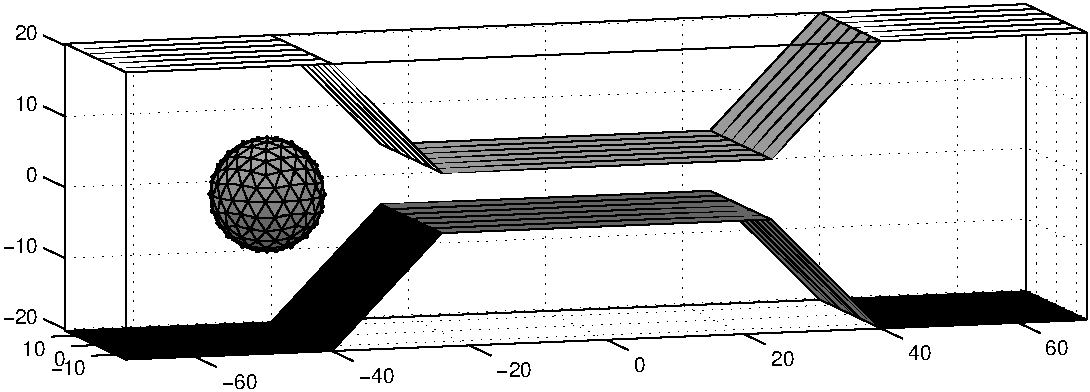
\includegraphics[width=\textwidth]{config.pdf}
}

\subsection{结果}
\frame{\frametitle{结果}
\begin{center}
  \animategraphics[width=1\textwidth, autoplay, loop]{5}{./animate/Cell/}{1}{109}
\end{center}
}

\frame{\frametitle{细胞构型}
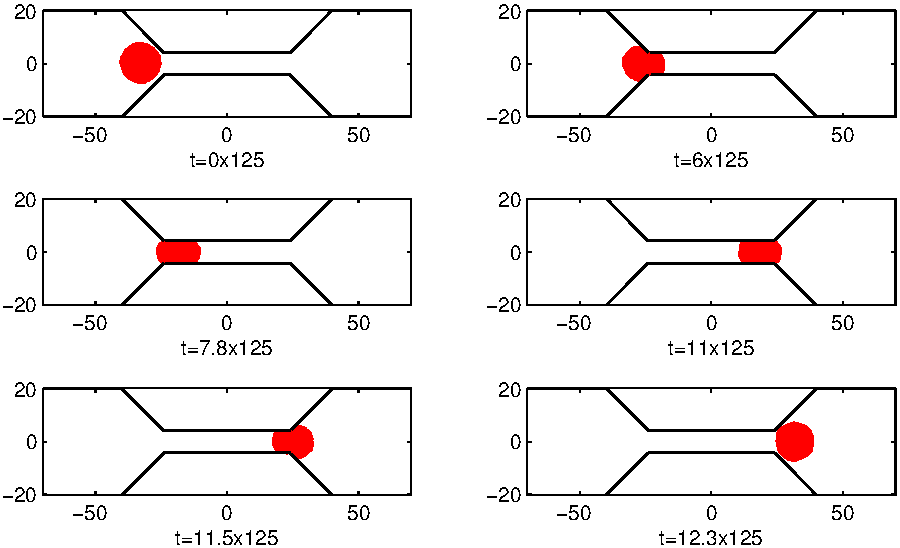
\includegraphics[width=1\textwidth]{cell.pdf}
}

\frame{\frametitle{位移与速度}
 \begin{columns}
  \begin{column}[b]{0.5\textwidth}
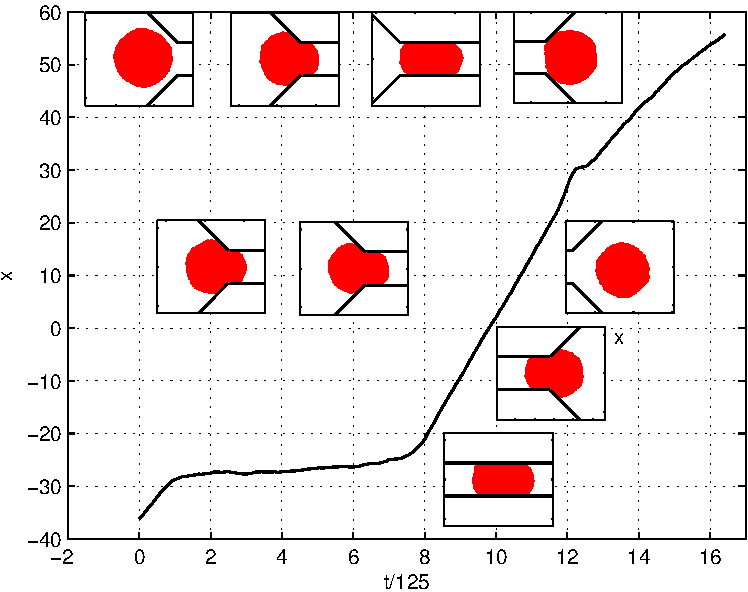
\includegraphics[width=1\textwidth]{x.pdf}
  \end{column}
  \begin{column}[b]{0.5\textwidth}
\begin{center}
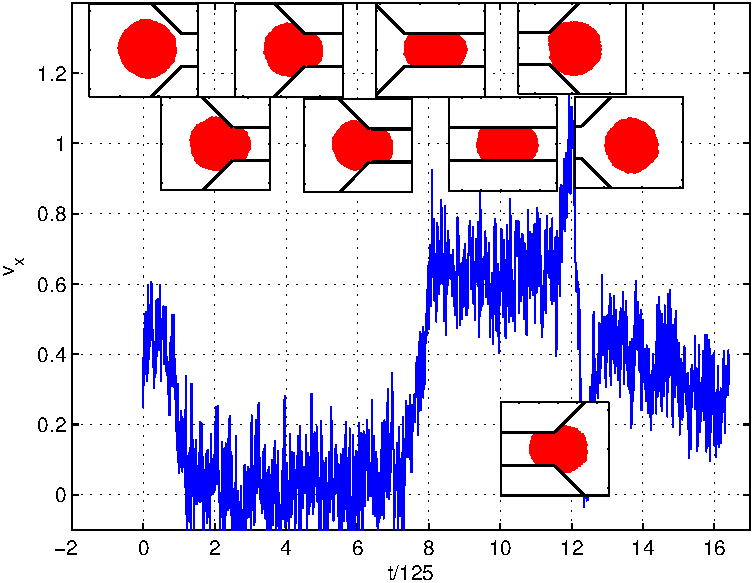
\includegraphics[width=1\textwidth]{cellLenght.pdf}
\end{center}
  \end{column}
\end{columns}
}

\frame{\frametitle{构型与实验对比}
 \begin{columns}
  \begin{column}[c]{0.5\textwidth}
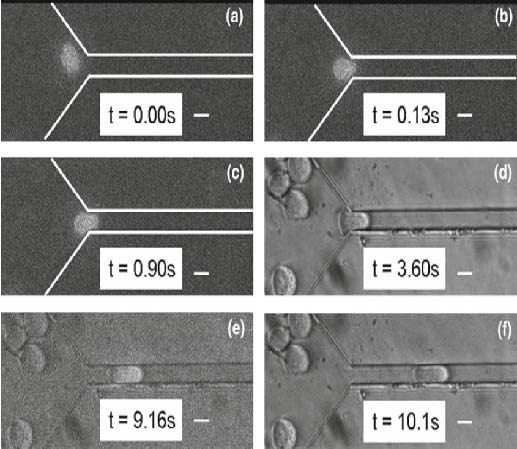
\includegraphics[width=\textwidth]{cell.jpg}
  \end{column}
  \begin{column}[c]{0.5\textwidth}
\begin{center}
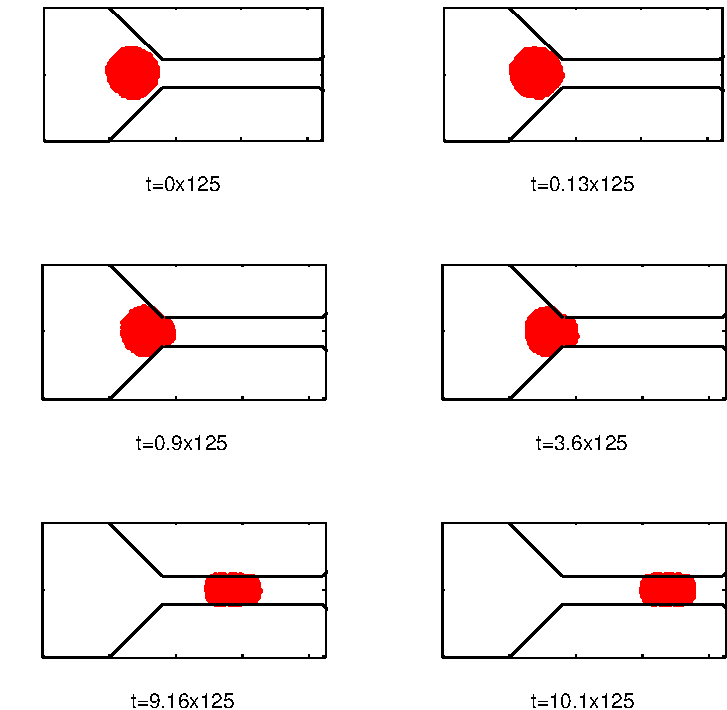
\includegraphics[width=0.98\textwidth]{cellconfig.pdf}
\end{center}
  \end{column}
\end{columns}
}

\frame{\frametitle{速度与实验对比}
 \begin{columns}
  \begin{column}[b]{0.46\textwidth}
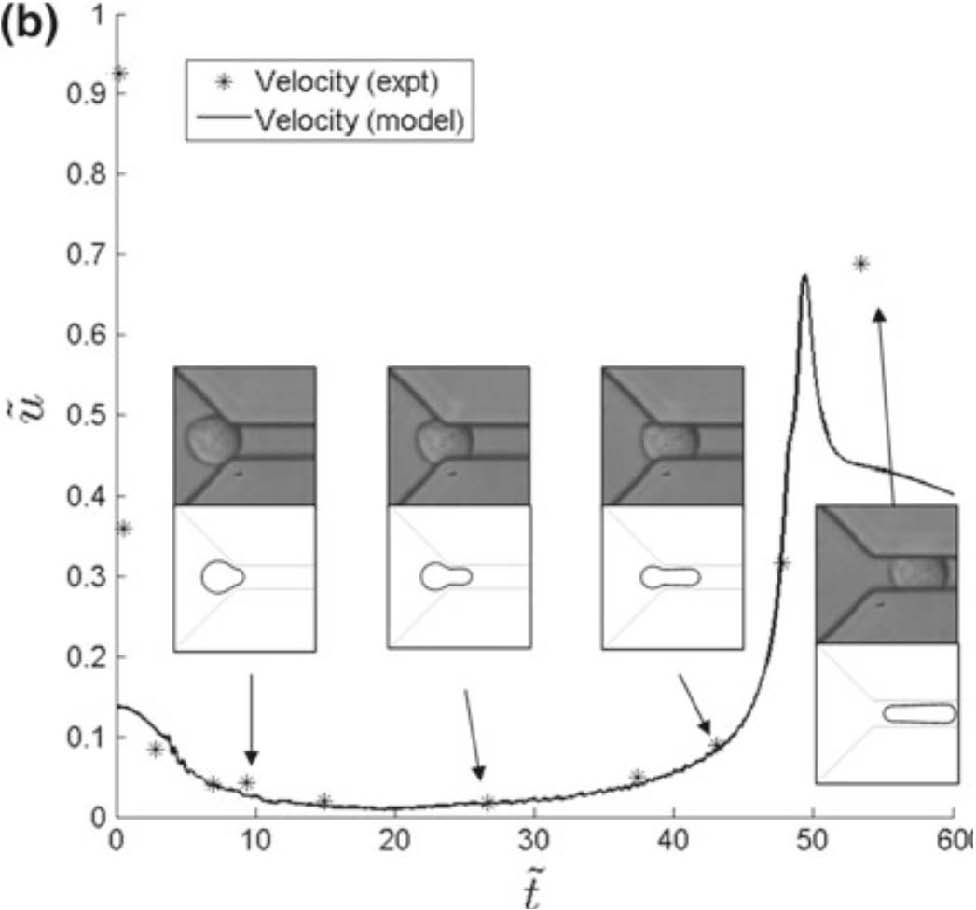
\includegraphics[width=1\textwidth]{vx.jpg}
  \end{column}
  \begin{column}[b]{0.54\textwidth}
\begin{center}
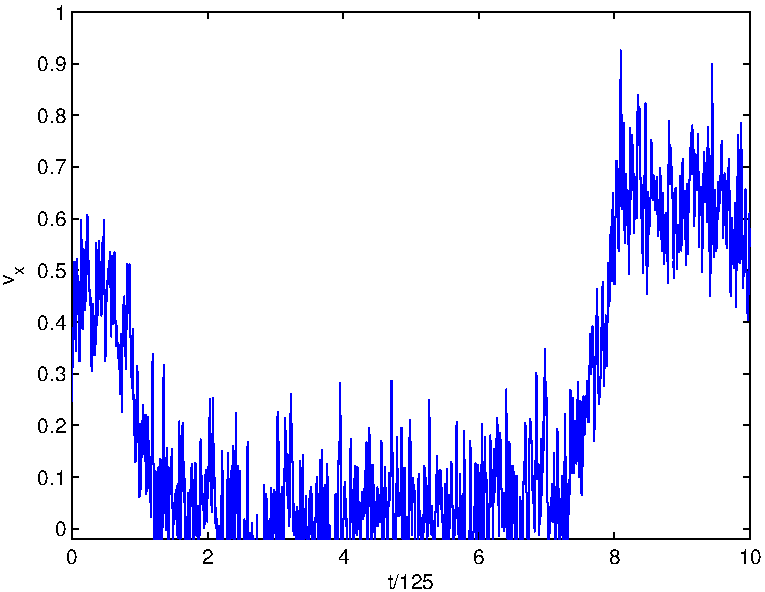
\includegraphics[width=1\textwidth]{vx.pdf}
\end{center}
  \end{column}
\end{columns}
}

\section{结论}
\frame{\frametitle{结论}
\begin{itemize}
\item 应用DPD方法及FENE珠簧链模型对细胞在微缩通道中的运动作了初步地模拟和尝试.模拟所得结果与实验基本吻合.
\item 本文的模型和模拟对于细胞的大变形和小变形都可以较好的模拟.
\item 细胞在开始进入微缩通道时减速, 拉长自身, 当细胞绝大部进入微缩结构后, 迅速加速直至细胞完全进入微缩通道; 细胞在微缩通道中的运动速度几乎不变. 当细胞从微缩结构的出口离开时, 又逐渐恢复了球形.  数值模拟所得到的细胞变形, 吸入及释放复原的形态与实验结果吻合.

\end{itemize}
}
